%%% In this section, you will describe all of the various artifacts that you will generate and maintain during the project life cycle. Describe the purpose of each item below, how the content will be generated, where it will be stored, how often it will be updated, etc. Replace the default text for each section with your own description. Reword this paragraph as appropriate.

\subsection{Major Documentation Deliverables}

\subsubsection{Project Charter}
This document will be updated once per week during the team's weekly meeting. Changes will be made any time the team makes a decision that change one of the subjects detailed in this document. The initial version will be submitted Tuesday, October 23, 2018. The final version will be delivered May 1, 2018.

\subsubsection{System Requirements Specification}
This document will be updated anytime a new portion is added to the project. It will also be updates if there is a portion of the system that is found faulty or not feasible to work with. The initial version will be delivered along with the first charter report while the final version will be delivered when the design of the system has been concluded on and no changes need to be made.

\subsubsection{Architectural Design Specification}
This document will be updated anytime a new portion is added to the project. It will also be updates if there is a portion of the system that is found faulty or not feasible to work with. The initial version will be delivered along with the first charter report while the final version will be delivered when the design of the system has been concluded on and no changes need to be made.

\subsubsection{Detailed Design Specification}
This document will be updated anytime a new portion is added to the project. It will also be updates if there is a portion of the system that is found faulty or not feasible to work with. The new changes will be described in detail showing what was removed or what was added in the design. The initial version will be delivered along with the first charter report while the final version will be delivered when the design of the system has been concluded on and no changes need to be made.

\subsection{Recurring Sprint Items}

\subsubsection{Product Backlog}
Team members will meet to determine requirements and break them down into features, which will be added to the backlog. Team members will determine the priority of each feature with a group vote, giving the most weight to items that progress development. The backlog will be a Google workbook document that can be edited and tracked by all team members.

\subsubsection{Sprint Planning}
At the end of one sprint there will be a meeting to discuss the next sprint. The backlog will be updated and tasks for each feature will be assigned. There will be 4 sprints, each lasting 3 weeks.

\subsubsection{Sprint Goal}
The team as a whole will determine the end goal of each sprint during the sprint planing meeting. The professor will be consulted periodically through the process via email and in-person communication. 

\subsubsection{Sprint Backlog}
The team as a whole will determine which backlog items are implemented into a sprint and when. The backlog will be a Google workbook document that can be edited and tracked by all team members.

\subsubsection{Task Breakdown}
The team will assign tasks during the sprint planing meeting. Team members can volunteer for tasks, or tasks can be assigned based on skill set. Task will be equally distributed across all members. Each team member will be responsible for tracking and recording the time spent on their assigned tasks. 

\subsubsection{Sprint Burn Down Charts}
Team members will alternate being scrum master. The scrum master will be responsible for monitoring the backlog. The backlog will generate a burn chart based on the data input into the table. Each team member will have access to update the backlog with the amount of time spent on each task. When this value is updated the burn chart will update the graph.

\begin{figure}[h!]
    \centering
    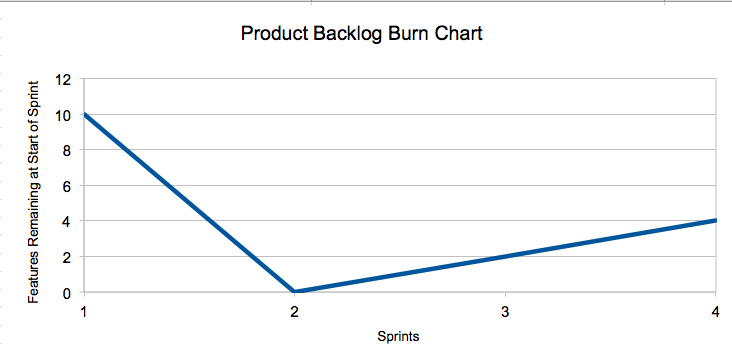
\includegraphics[width=0.5\textwidth]{images/burn_down_chart_example}
    \caption{Example sprint burn down chart}
\end{figure}

\subsubsection{Sprint Retrospective}
The sprint retrospective will take place at a team meeting. It will occur after every sprint has passed . The group will document what worked and should be maintained, what needs to improve and also resolve any conflict that arises in the just concluded sprint. It will be due about a week after the meeting has been held.

\subsubsection{Individual Status Reports}
Each member would report on any task that has been assigned to them to work on. It will be reported anytime there is a new task assigned and also when the report needs to be turned in. Every item assigned to each individual relating to the building of the project is considered a key item and should be added in the report.

\subsubsection{Engineering Notebooks}
The engineering notebook will be updated anytime work is done on the project. Therefore each member would always enter any part of the project they are working on. The minimum amount of pages as of now should be 1 page. Every section of the project assigned by the group is considered an interval so each interval is till the that section is finished. At least two other team members will sign the engineering notebooks as witnesses for each page.

\subsection{Closeout Materials}

\subsubsection{System Prototype}
The final system prototype will include a working haptic vest receiving data/information from a Raspberry Pi system, all of which can also be controlled through the Web interface. It is expected that the project will be demonstrated in person, at some point during the second semester. We expect to have several prototype acceptance tests with the customer, to ensure that the product is being made to their specifications. No off-site testing will be needed.

\subsubsection{Project Poster}
The poster will have a picture of the finished vest, as well as any basic schematics or blueprints we create. We will also give a quick summary of the vest's features, as well as any pertinent technical information.

\subsubsection{Web Page}
The website will be used to configure the settings of the vest, and select the music that will be processed by the vest. The site will be hosted on Hiroku, and it will be implemented using NoteJS, FireBase or MongoDB (for the database), and Express (for routing, if needed).

\subsubsection{Demo Video}
We do not expect that a demo video would be needed, if the project can be presented in person.

\subsubsection{Source Code}
Changes to the source code will be saved to the Github repository used to host the project. All source code will be freely available to the customer.

\subsubsection{Source Code Documentation}
The source code will be documented using Doxygen.

\subsubsection{Hardware Schematics}
At the time of writing, we have no hardware schematics.

\subsubsection{CAD files}
This is still to be determined.

\subsubsection{Installation Scripts}
This is still to be determined.

\subsubsection{User Manual}
The digital user manual that we expect to have will have basic instructions for wearing and using the vest, as well as instructions on how to properly set up the vest for use, including instructions for how to correctly run all the software.
